
\let\negmedspace\undefined
\let\negthickspace\undefined
\documentclass[journal,12pt,twocolumn]{IEEEtran}
\usepackage{cite}
\usepackage{amsmath,amssymb,amsfonts,amsthm}
\usepackage{algorithmic}
\usepackage{graphicx}
\usepackage{textcomp}
\usepackage{xcolor}
\usepackage{txfonts}
\usepackage{listings}
\usepackage{enumitem}
\usepackage{mathtools}
\usepackage{gensymb}
\usepackage[breaklinks=true]{hyperref}
\usepackage{tkz-euclide} % loads  TikZ and tkz-base
\usepackage{listings}
\usepackage{float}

\DeclareMathOperator*{\Res}{Res}
%\renewcommand{\baselinestretch}{2}
\renewcommand\thesection{\arabic{section}}
\renewcommand\thesubsection{\thesection.\arabic{subsection}}
\renewcommand\thesubsubsection{\thesubsection.\arabic{subsubsection}}

\renewcommand\thesectiondis{\arabic{section}}
\renewcommand\thesubsectiondis{\thesectiondis.\arabic{subsection}}
\renewcommand\thesubsubsectiondis{\thesubsectiondis.\arabic{subsubsection}}

% correct bad hyphenation here
\hyphenation{op-tical net-works semi-conduc-tor}
\def\inputGnumericTable{}                                 %%

\lstset{
%language=C,
frame=single, 
breaklines=true,
columns=fullflexible
}
%\lstset{
%language=tex,
%frame=single, 
%breaklines=true
%}

\begin{document}
%


\newtheorem{theorem}{Theorem}[section]
\newtheorem{problem}{Problem}
\newtheorem{proposition}{Proposition}[section]
\newtheorem{lemma}{Lemma}[section]
\newtheorem{corollary}[theorem]{Corollary}
\newtheorem{example}{Example}[section]
\newtheorem{definition}[problem]{Definition}
%\newtheorem{thm}{Theorem}[section] 
%\newtheorem{defn}[thm]{Definition}
%\newtheorem{algorithm}{Algorithm}[section]
%\newtheorem{cor}{Corollary}
\newcommand{\BEQA}{\begin{eqnarray}}
\newcommand{\EEQA}{\end{eqnarray}}
\newcommand{\define}{\stackrel{\triangle}{=}}

\bibliographystyle{IEEEtran}
%\bibliographystyle{ieeetr}


\providecommand{\mbf}{\mathbf}
\providecommand{\pr}[1]{\ensuremath{\Pr\left(#1\right)}}
\providecommand{\qfunc}[1]{\ensuremath{Q\left(#1\right)}}
\providecommand{\sbrak}[1]{\ensuremath{{}\left[#1\right]}}
\providecommand{\lsbrak}[1]{\ensuremath{{}\left[#1\right.}}
\providecommand{\rsbrak}[1]{\ensuremath{{}\left.#1\right]}}
\providecommand{\brak}[1]{\ensuremath{\left(#1\right)}}
\providecommand{\lbrak}[1]{\ensuremath{\left(#1\right.}}
\providecommand{\rbrak}[1]{\ensuremath{\left.#1\right)}}
\providecommand{\cbrak}[1]{\ensuremath{\left\{#1\right\}}}
\providecommand{\lcbrak}[1]{\ensuremath{\left\{#1\right.}}
\providecommand{\rcbrak}[1]{\ensuremath{\left.#1\right\}}}
\theoremstyle{remark}
\newtheorem{rem}{Remark}
\newcommand{\sgn}{\mathop{\mathrm{sgn}}}
\providecommand{\abs}[1]{\left\vert#1\right\vert}
\providecommand{\res}[1]{\Res\displaylimits_{#1}} 
\providecommand{\norm}[1]{\left\lVert#1\right\rVert}
%\providecommand{\norm}[1]{\lVert#1\rVert}
\providecommand{\mtx}[1]{\mathbf{#1}}
\providecommand{\mean}[1]{E\left[ #1 \right]}
\providecommand{\fourier}{\overset{\mathcal{F}}{ \rightleftharpoons}}
%\providecommand{\hilbert}{\overset{\mathcal{H}}{ \rightleftharpoons}}
\providecommand{\system}{\overset{\mathcal{H}}{ \longleftrightarrow}}
	%\newcommand{\solution}[2]{\textbf{Solution:}{#1}}
\newcommand{\solution}{\noindent \textbf{Solution: }}
\newcommand{\cosec}{\,\text{cosec}\,}
\providecommand{\dec}[2]{\ensuremath{\overset{#1}{\underset{#2}{\gtrless}}}}
\newcommand{\myvec}[1]{\ensuremath{\begin{pmatrix}#1\end{pmatrix}}}
\newcommand{\mydet}[1]{\ensuremath{\begin{vmatrix}#1\end{vmatrix}}}

\let\vec\mathbf

\vspace{3cm}

\title{
\textbf{Bonus Question} \\ \large \textbf{AI1110}: Probability and Random Variables 


}
\author{ Rishitha Surineni\\ cs22btech11050} 

% make the title area
\maketitle

\newpage

%\tableofcontents

\bigskip

\renewcommand{\thefigure}{\theenumi}
\renewcommand{\thetable}{\theenumi}

\textbf{Question:}\\
 	It is known that $ 10\% $ of certain articles manufactured are defective.What is the probability that in a random sample space of 12 such articles, 9 are defective?
\\
 \textbf{Solution:}
 \\
Let $X_i$ be a random variable corresponding to $i^{th}$ article such that
\begin{align}
        X_i=  
        \begin{cases}
            1 &  \text{if the article is defective} \\
            0 &  \text{if the article is not defective}
        \end{cases}
    \end{align}
\\$X_1,X_2,...,X_{12}$ is a sequence of independent and identically distributed random variables.This sequence forms a Binomial Distribution with mean $\mu$ and variance $\sigma^2$
 \\For this Binomial Distribution, n = 12 and p = 0.1.
 \\The mean and standard deviation of the Binomial distribution are
 \begin{align}
    \mu &= np\\
    \mu &= 12\times0.1\\
    \mu &= 1.2\\
    \sigma&= \sqrt{np(1-p)}\\
    \sigma&= \sqrt{12\times0.1\times0.9}\\
    \sigma&= 1.04
    \end{align}
Let $S_n = \sum_{i=1}^{n} X_i$
\begin{align}
      \text{Standardized sample mean} = \frac{\frac{S_n}{n}-\mu}{\frac{\sigma}{\sqrt{n}}} \\
      = \frac{S_n-\mu{n}}{\sigma{\sqrt{n}}} 
    \end{align}
as $n \to \infty$ ,$\frac{S_n -\mu{n}}{\sigma{\sqrt{n}}} \to N(0,1)$
\\here N(0,1) denotes a standard normal distribution with mean 0 and variance 1.
 \\Let, E be the event that exactly 9 articles are defective.
 \\For the event E
 \begin{align}
    S_n &= 9 \text{[as exactly 9 articles are defective]}\nonumber\\
    &\text{Standardized sample mean for the event E is} \nonumber\\
    z &= \frac{S_n-np}{\sqrt{np(1-p)}}\\
    z &= \frac{9-1.2}{1.04}\\
    z &= 7.5
    \end{align}
From the Standard Normal Distribution table,
\\The probability of an event having standardized sample mean value than 7.5 is very low and is equal to $4.338751580235112 \times 10^{-13}$
\\Therefore, $\pr{E} = 4.338751580235112 \times 10^{-13}$
\begin{figure}[h]
\centering
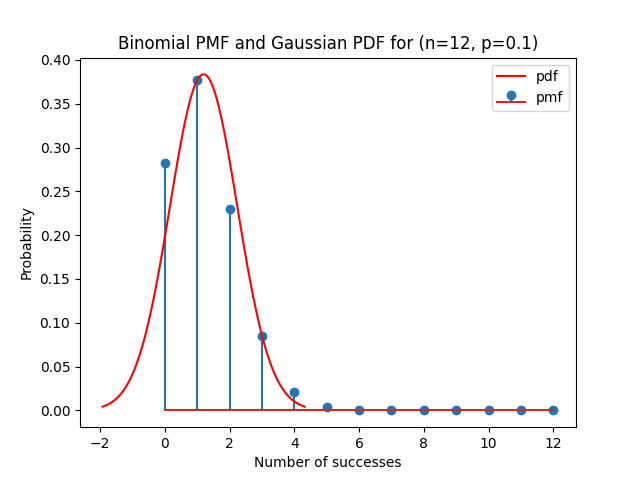
\includegraphics[width=\columnwidth]{./figs/graph.png}
\end{figure}
\end {document}